\documentclass[11pt,a4paper]{report}
\usepackage[textwidth=37em,vmargin=30mm]{geometry}
\usepackage{calc,xunicode,amsmath,amssymb,paralist,enumitem,tabu,booktabs,datetime2,xeCJK,xeCJKfntef,listings}
\usepackage{tocloft,fancyhdr,tcolorbox,xcolor,graphicx,eso-pic,xltxtra,xelatexemoji}

\newcommand{\envyear}[0]{2025}
\newcommand{\envdatestr}[0]{2025-06-11}
\newcommand{\envfinaldir}[0]{webdb/2025/20250611/final}

\usepackage[hidelinks]{hyperref}
\hypersetup{
    colorlinks=false,
    pdfpagemode=FullScreen,
    pdftitle={Web Digest - \envdatestr}
}

\setlength{\cftbeforechapskip}{10pt}
\renewcommand{\cftchapfont}{\rmfamily\bfseries\large\raggedright}
\setlength{\cftbeforesecskip}{2pt}
\renewcommand{\cftsecfont}{\sffamily\small\raggedright}

\setdefaultleftmargin{2em}{2em}{1em}{1em}{1em}{1em}

\usepackage{xeCJK,xeCJKfntef}
\xeCJKsetup{PunctStyle=plain,RubberPunctSkip=false,CJKglue=\strut\hskip 0pt plus 0.1em minus 0.05em,CJKecglue=\strut\hskip 0.22em plus 0.2em}
\XeTeXlinebreaklocale "zh"
\XeTeXlinebreakskip = 0pt


\setmainfont{Brygada 1918}
\setromanfont{Brygada 1918}
\setsansfont{IBM Plex Sans}
\setmonofont{JetBrains Mono NL}
\setCJKmainfont{Noto Serif CJK SC}
\setCJKromanfont{Noto Serif CJK SC}
\setCJKsansfont{Noto Sans CJK SC}
\setCJKmonofont{Noto Sans CJK SC}

\setlength{\parindent}{0pt}
\setlength{\parskip}{8pt}
\linespread{1.15}

\lstset{
	basicstyle=\ttfamily\footnotesize,
	numbersep=5pt,
	backgroundcolor=\color{black!5},
	showspaces=false,
	showstringspaces=false,
	showtabs=false,
	tabsize=2,
	captionpos=b,
	breaklines=true,
	breakatwhitespace=true,
	breakautoindent=true,
	linewidth=\textwidth
}






\newcommand{\coverpic}[2]{
    % argv: itemurl, authorname
    Cover photo by #2~~(\href{#1}{#1})
}
\newcommand{\makeheader}[0]{
    \begin{titlepage}
        % \newgeometry{hmargin=15mm,tmargin=21mm,bmargin=12mm}
        \begin{center}
            
            \rmfamily\scshape
            \fontspec{BaskervilleF}
            \fontspec{Old Standard}
            \fontsize{59pt}{70pt}\selectfont
            WEB\hfill DIGEST
            
            \vfill
            % \vskip 30pt
            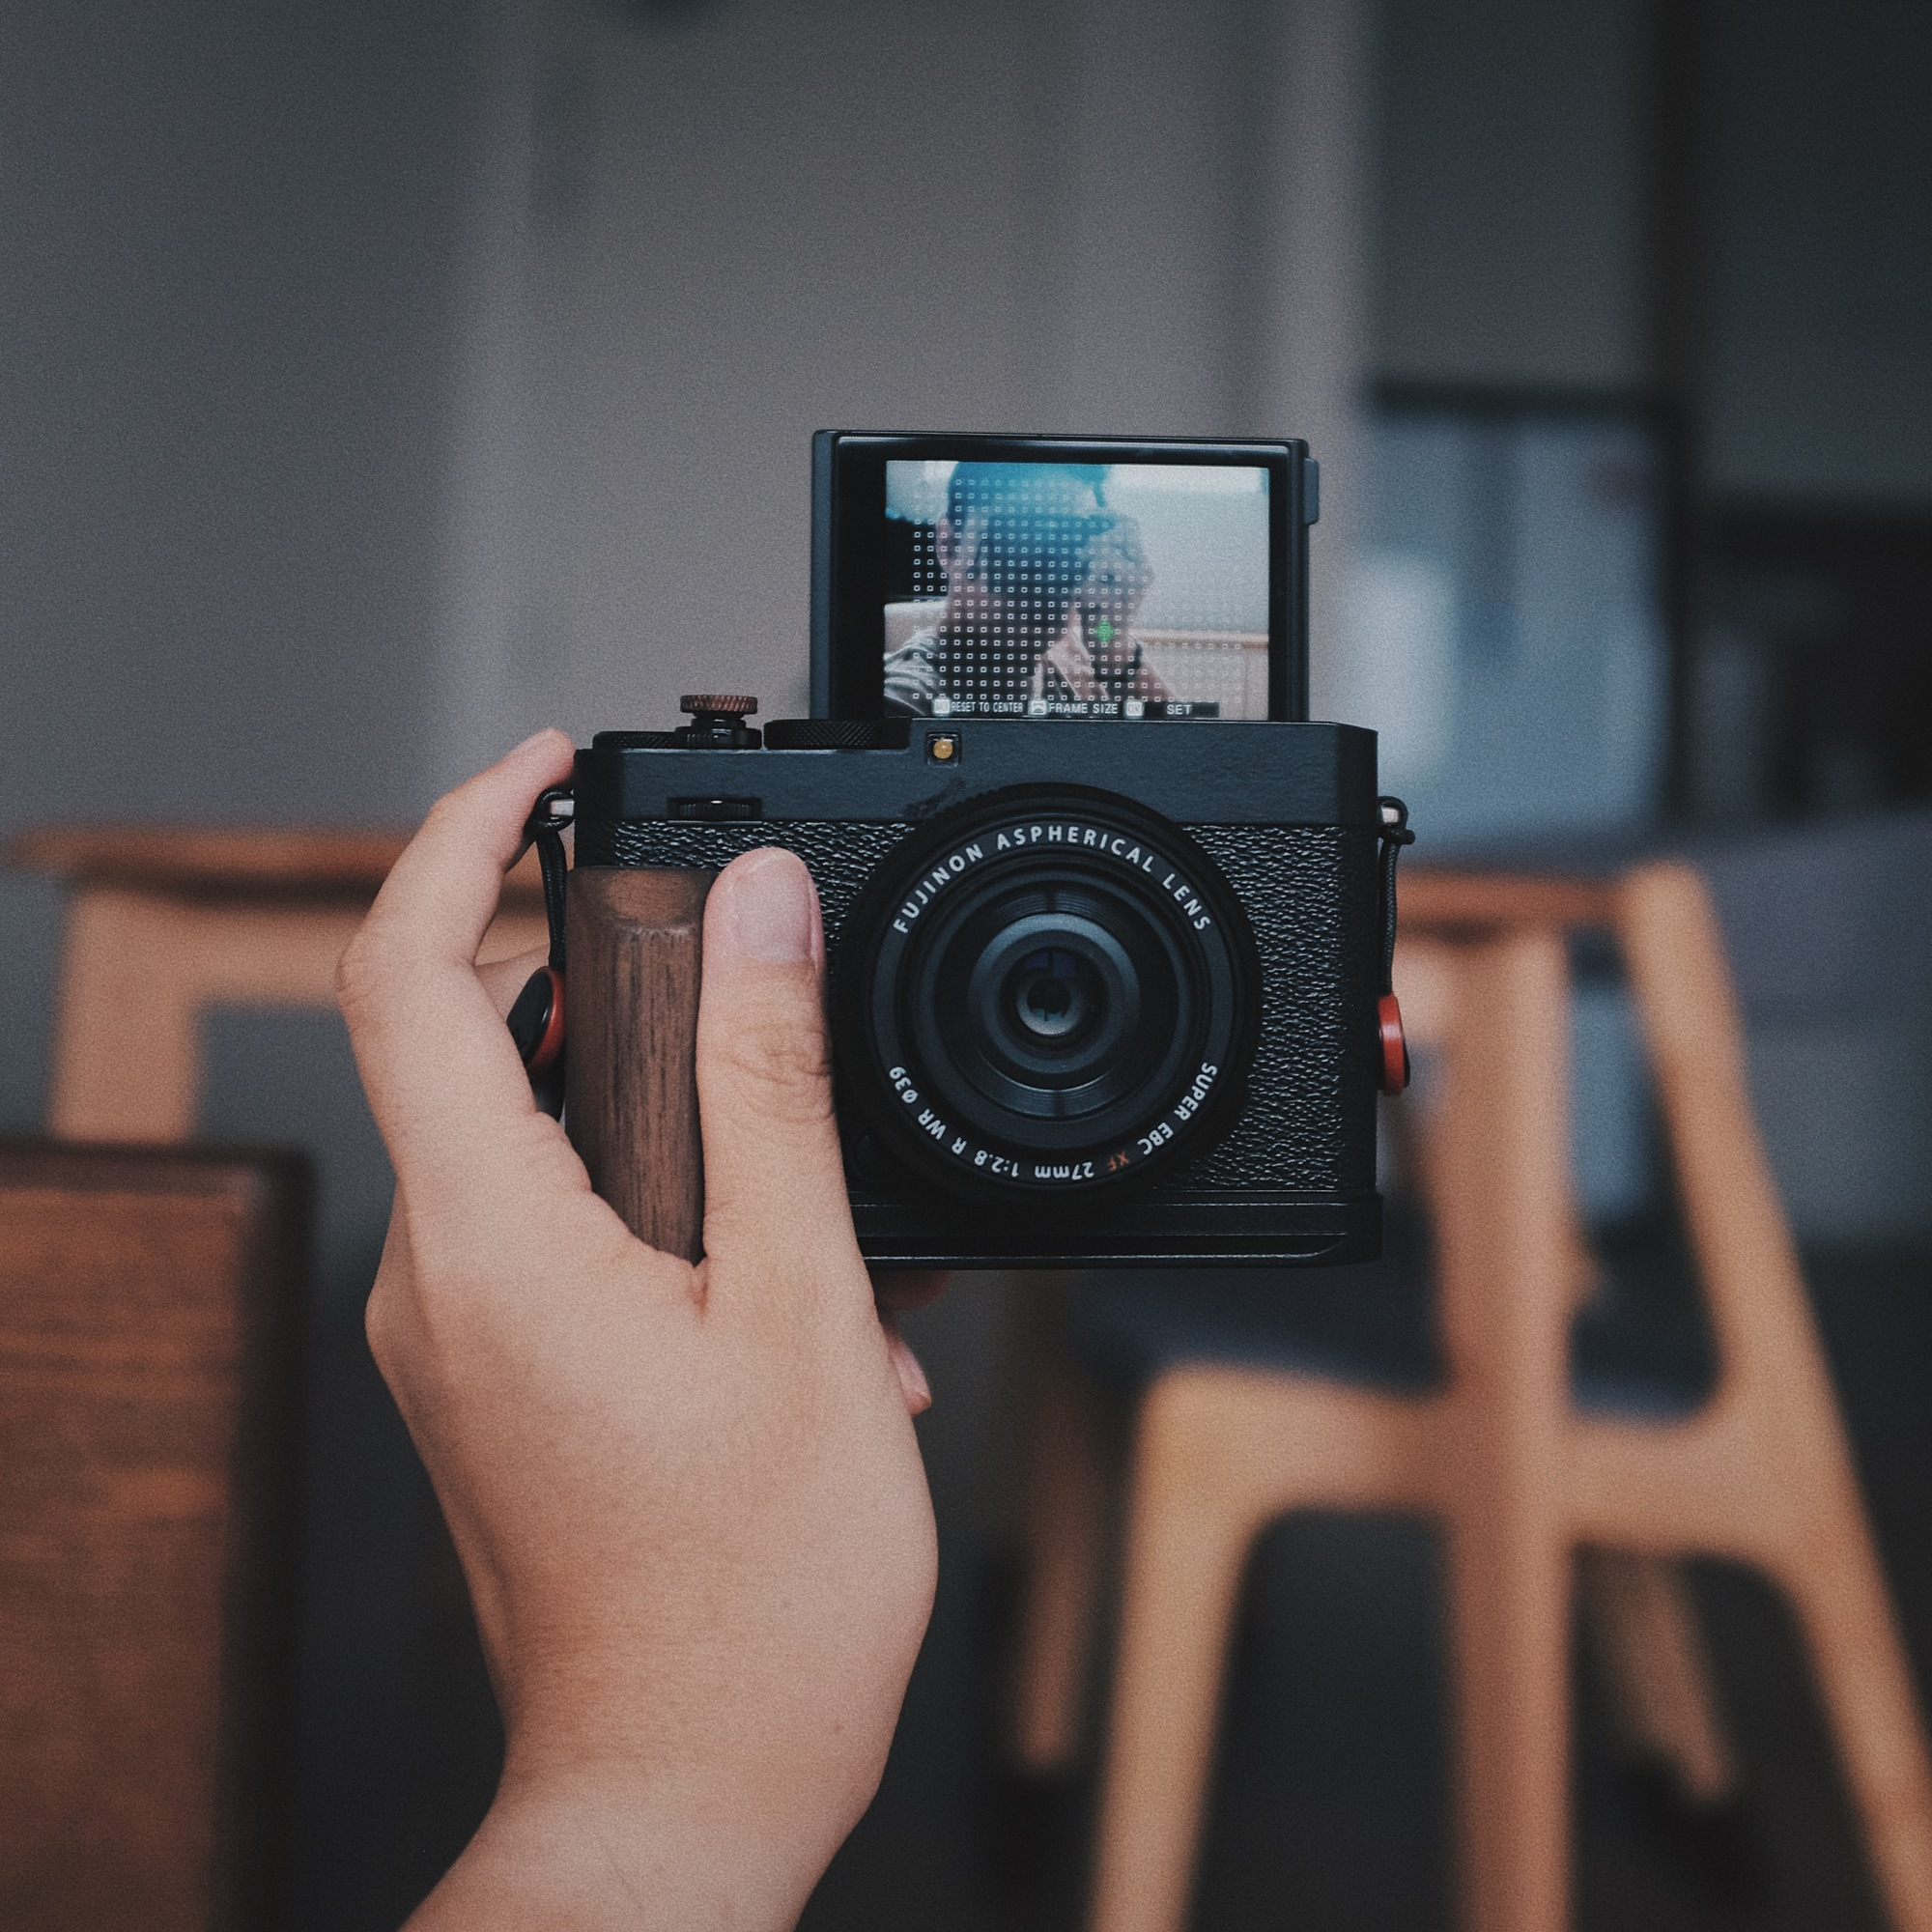
\includegraphics[width=\linewidth]{\envfinaldir/coverpic-prod.jpg}\par
            % \vskip 30pt
            \vfill

            \normalsize\rmfamily\scshape
            \copyright{} The Web Digest Project \hfill\large \envdatestr
        \end{center}
    \end{titlepage}
    % \restoregeometry
}
\newcommand{\simplehref}[1]{%
    \textcolor{blue!80!green}{\href{#1}{#1}}%
}
\renewcommand{\contentsname}{\center\Huge\sffamily\bfseries Contents\par\vskip 20pt}
\newcounter{ipartcounter}
\setcounter{ipartcounter}{0}
\newcommand{\ipart}[1]{
    % \vskip 20pt
    \clearpage
    \stepcounter{ipartcounter}
    \phantomsection
    \addcontentsline{toc}{chapter}{#1}
    % \begin{center}
    %     \Huge
    %     \sffamily\bfseries
    %     #1
    % \end{center}
    % \vskip 20pt plus 7pt
}
\newcounter{ichaptercounter}
\setcounter{ichaptercounter}{0}
\newcommand{\ichapter}[1]{
    % \vskip 20pt
    \clearpage
    \stepcounter{ichaptercounter}
    \phantomsection
    \addcontentsline{toc}{section}{\numberline{\arabic{ichaptercounter}}#1}
    \begin{center}
        \Huge
        \sffamily\bfseries
        #1
    \end{center}
    \vskip 20pt plus 7pt
}
\newcommand{\entrytitlefont}[1]{\subsection*{\raggedright\Large\sffamily\bfseries#1}}
\newcommand{\entryitemGeneric}[2]{
    % argv: title, url
    \parbox{\linewidth}{
        \entrytitlefont{#1}\par\vskip 5pt
        \footnotesize\ttfamily\mdseries
        \simplehref{#2}
    }\vskip 11pt plus 11pt minus 1pt
}
\newcommand{\entryitemGithub}[3]{
    % argv: title, url, desc
    \parbox{\linewidth}{
        \entrytitlefont{#1}\par\vskip 5pt
        \footnotesize\ttfamily\mdseries
        \simplehref{#2}\par\vskip 5pt
        \small\rmfamily\mdseries#3
    }\vskip 11pt plus 11pt minus 1pt
}
\newcommand{\entryitemAp}[3]{
    % argv: title, url, desc
    \parbox{\linewidth}{
        \entrytitlefont{#1}\par\vskip 5pt
        \footnotesize\ttfamily\mdseries
        \simplehref{#2}\par\vskip 5pt
        \small\rmfamily\mdseries#3
    }\vskip 11pt plus 11pt minus 1pt
}
\newcommand{\entryitemHackernews}[3]{
    % argv: title, hnurl, rawurl
    % \parbox{\linewidth}{
    %     \entrytitlefont{#1}\par\vskip 5pt
    %     \footnotesize\ttfamily\mdseries
    %     \simplehref{#3}\par
    %     \textcolor{black!50}{\href{#2}{#2}}
    % }\vskip 11pt plus 11pt minus 1pt
    \begin{minipage}{\linewidth}
            \entrytitlefont{#1}\par\vskip 5pt
            \footnotesize\ttfamily\mdseries
            \simplehref{#3}\par
            \textcolor{black!50}{\href{#2}{#2}}
    \end{minipage}\par\vskip 11pt plus 11pt minus 1pt
}







\begin{document}

\makeheader

\tableofcontents\clearpage




\ipart{Developers}
\ichapter{Hacker News}
\entryitemTwoLinks{Show HN: I made a 3D printed VTOL drone}{https://news.ycombinator.com/item?id=44241278}{https://www.tsungxu.com/p/i-made-a-3d-printed-vtol-that-can}

\entryitemTwoLinks{OpenAI o3-pro}{https://news.ycombinator.com/item?id=44240999}{https://help.openai.com/en/articles/9624314-model-release-notes}

\entryitemTwoLinks{Launch HN: Vassar Robotics (YC X25) – \$219 robot arm that learns new skills}{https://news.ycombinator.com/item?id=44240302}{https://news.ycombinator.com/item?id=44240302}

\entryitemTwoLinks{Android 16 is here}{https://news.ycombinator.com/item?id=44239812}{https://blog.google/products/android/android-16/}

\entryitemTwoLinks{Low-background Steel: content without AI contamination}{https://news.ycombinator.com/item?id=44239481}{https://blog.jgc.org/2025/06/low-background-steel-content-without-ai.html}

\entryitemTwoLinks{OpenAI dropped the price of o3 by 80\%}{https://news.ycombinator.com/item?id=44239359}{https://twitter.com/sama/status/1932434606558462459}

\entryitemTwoLinks{Show HN: Chili3d – A open-source, browser-based 3D CAD application}{https://news.ycombinator.com/item?id=44238171}{https://news.ycombinator.com/item?id=44238171}

\entryitemTwoLinks{Malleable software: Restoring user agency in a world of locked-down apps}{https://news.ycombinator.com/item?id=44237881}{https://www.inkandswitch.com/essay/malleable-software/}

\entryitemTwoLinks{Magistral — the first reasoning model by Mistral AI}{https://news.ycombinator.com/item?id=44236997}{https://mistral.ai/news/magistral}

\entryitemTwoLinks{Show HN: PyDoll – Async Python scraping engine with native CAPTCHA bypass}{https://news.ycombinator.com/item?id=44236926}{https://github.com/autoscrape-labs/pydoll}

\entryitemTwoLinks{Finding Atari Games in Randomly Generated Data}{https://news.ycombinator.com/item?id=44236900}{https://bbenchoff.github.io/pages/FiniteAtari.html}

\entryitemTwoLinks{Mikeal Rogers has died}{https://news.ycombinator.com/item?id=44236728}{https://b.h4x.zip/mikeal/}

\entryitemTwoLinks{Faster, easier 2D vector rendering [video]}{https://news.ycombinator.com/item?id=44236423}{https://www.youtube.com/watch?v=\_sv8K190Zps}

\entryitemTwoLinks{Show HN: High End Color Quantizer}{https://news.ycombinator.com/item?id=44235628}{https://github.com/big-nacho/patolette}

\entryitemTwoLinks{"Localhost tracking" explained. It could cost Meta €32B}{https://news.ycombinator.com/item?id=44235467}{https://www.zeropartydata.es/p/localhost-tracking-explained-it-could}

\entryitemTwoLinks{WWDC25: macOS Tahoe Breaks Decades of Finder History}{https://news.ycombinator.com/item?id=44235177}{https://512pixels.net/2025/06/wwdc25-macos-tahoe-breaks-decades-of-finder-history/}

\entryitemTwoLinks{The Danish Ministry of Digitalization Is Switching to Linux and LibreOffice}{https://news.ycombinator.com/item?id=44234552}{https://politiken.dk/viden/tech/art10437680/Caroline-Stage-udfaser-Microsoft-i-Digitaliseringsministeriet}

\entryitemTwoLinks{Denmark: Minister for Digitalization wants to phase out Microsoft}{https://news.ycombinator.com/item?id=44234290}{https://nordjyske.dk/nyheder/politik/digitaliseringsminister-vil-udfase-microsoft-i-sit-eget-ministerium/5616096}

\entryitemTwoLinks{Europe needs digital sovereignty – and Microsoft has just proven why}{https://news.ycombinator.com/item?id=44233480}{https://tuta.com/blog/digital-sovereignty-europe}

\entryitemTwoLinks{Successful people set constraints rather than chasing goals}{https://news.ycombinator.com/item?id=44232714}{https://www.joanwestenberg.com/smart-people-dont-chase-goals-they-create-limits/}\ichapter{Dribbble}
\entryitemGeneric{\hskip 0pt{}Aquasan}{https://dribbble.com/shots/26100535-Aquasan}

\entryitemGeneric{\hskip 0pt{}Eagle}{https://dribbble.com/shots/26099428-Eagle}

\entryitemGeneric{\hskip 0pt{}Mnp Technologies - Logo Design}{https://dribbble.com/shots/26092034-Mnp-Technologies-Logo-Design}

\entryitemGeneric{\hskip 0pt{}Singular Logo Concept (Unused)}{https://dribbble.com/shots/26091755-Singular-Logo-Concept-Unused}

\entryitemGeneric{\hskip 0pt{}Cre8tera // Website}{https://dribbble.com/shots/26091009-Cre8tera-Website}

\entryitemGeneric{\hskip 0pt{}Cool Pool Logo Design - Letter C Monogram}{https://dribbble.com/shots/26091401-Cool-Pool-Logo-Design-Letter-C-Monogram}

\entryitemGeneric{\hskip 0pt{}Gorilla + Bar Chart Logo}{https://dribbble.com/shots/26092670-Gorilla-Bar-Chart-Logo}

\entryitemGeneric{\hskip 0pt{}zeero logo design}{https://dribbble.com/shots/26087342-zeero-logo-design}

\entryitemGeneric{\hskip 0pt{}Create email inbox composition}{https://dribbble.com/shots/26083118-Create-email-inbox-composition}

\entryitemGeneric{\hskip 0pt{}Shori Brand}{https://dribbble.com/shots/26088139-Shori-Brand}

\entryitemGeneric{\hskip 0pt{}Roaring Bear}{https://dribbble.com/shots/26087788-Roaring-Bear}

\entryitemGeneric{\hskip 0pt{}Eagle}{https://dribbble.com/shots/26085536-Eagle}

\entryitemGeneric{\hskip 0pt{}Hand-drawn illustration pack}{https://dribbble.com/shots/26084735-Hand-drawn-illustration-pack}

\entryitemGeneric{\hskip 0pt{}Dog Mascot Various Poses}{https://dribbble.com/shots/26087977-Dog-Mascot-Various-Poses}

\entryitemGeneric{\hskip 0pt{}Branding Concept for Europe}{https://dribbble.com/shots/26087652-Branding-Concept-for-Europe}

\entryitemGeneric{\hskip 0pt{}B2B Dashboard \& Web App UI UX Design for Carbon Solutions}{https://dribbble.com/shots/26076624-B2B-Dashboard-Web-App-UI-UX-Design-for-Carbon-Solutions}

\entryitemGeneric{\hskip 0pt{}Patriot Logo Design (Unused for Sale)}{https://dribbble.com/shots/26081047-Patriot-Logo-Design-Unused-for-Sale}

\entryitemGeneric{\hskip 0pt{}Heliopoint}{https://dribbble.com/shots/26081987-Heliopoint}

\entryitemGeneric{\hskip 0pt{}Apple}{https://dribbble.com/shots/26084067-Apple}

\entryitemGeneric{\hskip 0pt{}Illustration}{https://dribbble.com/shots/26083223-Illustration}

\entryitemGeneric{\hskip 0pt{}Europe Logo Animation}{https://dribbble.com/shots/26082596-Europe-Logo-Animation}

\entryitemGeneric{\hskip 0pt{}Arc Logo}{https://dribbble.com/shots/26083648-Arc-Logo}

\entryitemGeneric{\hskip 0pt{}Heyo Turns 2!}{https://dribbble.com/shots/26078572-Heyo-Turns-2}

\entryitemGeneric{\hskip 0pt{}Fox Brand Mascot}{https://dribbble.com/shots/26077954-Fox-Brand-Mascot}


\ipart{Developers~~~~(zh-Hans)}
\ichapter{Solidot}
\entryitemGeneric{\hskip 0pt{}中国 AI 公司在高考期间短暂禁用了部分功能以防止考试作弊}{https://www.solidot.org/story?sid=81519}

\entryitemGeneric{\hskip 0pt{}欧洲需要数字主权}{https://www.solidot.org/story?sid=81518}

\entryitemGeneric{\hskip 0pt{}Mozilla 又关闭了两项服务}{https://www.solidot.org/story?sid=81517}

\entryitemGeneric{\hskip 0pt{}macOS Tahoe 将是最后一个支持英特尔处理器的 macOS 版本}{https://www.solidot.org/story?sid=81516}

\entryitemGeneric{\hskip 0pt{}按摩脸部和颈部或有助于大脑冲掉垃圾}{https://www.solidot.org/story?sid=81515}

\entryitemGeneric{\hskip 0pt{}人类昼夜节律与季节性阳光相关}{https://www.solidot.org/story?sid=81514}

\entryitemGeneric{\hskip 0pt{}拉斯维加斯的应对气候策略:种植更多树}{https://www.solidot.org/story?sid=81513}

\entryitemGeneric{\hskip 0pt{}报告称全球生育率普遍下滑}{https://www.solidot.org/story?sid=81512}

\entryitemGeneric{\hskip 0pt{}FAA 计划淘汰软盘和 Windows 95}{https://www.solidot.org/story?sid=81511}

\entryitemGeneric{\hskip 0pt{}印度 Manipur 邦实行宵禁并切断互联网访问}{https://www.solidot.org/story?sid=81509}

\entryitemGeneric{\hskip 0pt{}Linux 基金会试图和解围绕 WordPress 的纠纷}{https://www.solidot.org/story?sid=81508}

\entryitemGeneric{\hskip 0pt{}安全阻碍了企业拥抱 AI}{https://www.solidot.org/story?sid=81506}

\entryitemGeneric{\hskip 0pt{}谷歌CEO皮查伊:为什么说AI意义将超越火与电?}{https://www.solidot.org/story?sid=81505}

\entryitemGeneric{\hskip 0pt{}Google 塑造的 Web 也许将被重塑}{https://www.solidot.org/story?sid=81504}

\entryitemGeneric{\hskip 0pt{}微软第一方游戏进入 80 美元时代}{https://www.solidot.org/story?sid=81503}

\entryitemGeneric{\hskip 0pt{}Linux 6.16-rc1 释出}{https://www.solidot.org/story?sid=81502}

\entryitemGeneric{\hskip 0pt{}微软和华硕合作推出 Xbox 掌机 ROG Xbox Ally}{https://www.solidot.org/story?sid=81501}

\entryitemGeneric{\hskip 0pt{}Kagi 用户数突破五万}{https://www.solidot.org/story?sid=81500}

\entryitemGeneric{\hskip 0pt{}欧盟新规定强制要求为智能手机和平板提供五年操作系统更新}{https://www.solidot.org/story?sid=81499}

\entryitemGeneric{\hskip 0pt{}/e/OS 3.0 释出}{https://www.solidot.org/story?sid=81498}\ichapter{V2EX}
\entryitemGeneric{\hskip 0pt{}[问与答] 25 周岁了,没这么迷茫过,求教职业方向}{https://www.v2ex.com/t/1137781}

\entryitemGeneric{\hskip 0pt{}[分享创造] 完全免费,发布一个使用大模型帮高中生(北美)撰写 College Essay 的工具}{https://www.v2ex.com/t/1137779}

\entryitemGeneric{\hskip 0pt{}[程序员] meta 对中国市场到底有什么执念 恶心}{https://www.v2ex.com/t/1137777}

\entryitemGeneric{\hskip 0pt{}[OpenAI] 现在大陆通过机场使用 ChatGPT 还降智么?}{https://www.v2ex.com/t/1137776}

\entryitemGeneric{\hskip 0pt{}[Apple] 分享一个隐藏刘海的方法}{https://www.v2ex.com/t/1137775}

\entryitemGeneric{\hskip 0pt{}[宽带症候群] 家宽限速的颗粒是多大?}{https://www.v2ex.com/t/1137774}

\entryitemGeneric{\hskip 0pt{}[酷工作] 厦门保沣 制造业 信息部 招 后端工程师 new}{https://www.v2ex.com/t/1137773}

\entryitemGeneric{\hskip 0pt{}[Apple] Apple TV 26 系统支持音频直通}{https://www.v2ex.com/t/1137772}

\entryitemGeneric{\hskip 0pt{}[问与答] 想投资一张 5090 玩玩 AI 请问主机需要什么配置?}{https://www.v2ex.com/t/1137771}

\entryitemGeneric{\hskip 0pt{}[奇思妙想] 中国没有 AI 问诊的平台吗}{https://www.v2ex.com/t/1137769}

\entryitemGeneric{\hskip 0pt{}[宽带症候群] 记录一个很难绷的 ipv6 获取不到的问题}{https://www.v2ex.com/t/1137768}

\entryitemGeneric{\hskip 0pt{}[DNS] doh 能被运营商劫持吗}{https://www.v2ex.com/t/1137767}

\entryitemGeneric{\hskip 0pt{}[分享创造] [折腾记] 使用 Claude 开发一款宝宝双语认知卡片微信小程序}{https://www.v2ex.com/t/1137766}

\entryitemGeneric{\hskip 0pt{}[分享发现] Alist 似乎被卖了}{https://www.v2ex.com/t/1137764}

\entryitemGeneric{\hskip 0pt{}[奇思妙想] 你我之间,谁为真实?}{https://www.v2ex.com/t/1137762}

\entryitemGeneric{\hskip 0pt{}[生活] 求推荐靠谱免费的有声书分享渠道}{https://www.v2ex.com/t/1137761}

\entryitemGeneric{\hskip 0pt{}[程序员] 哪个大模型可以自动根据上下文生成关于某个主题的聊天对话(纯文本),同时在保持文字意思大致不变的前提下,精确嵌入隐藏水印?}{https://www.v2ex.com/t/1137758}

\entryitemGeneric{\hskip 0pt{}[问与答] 自己搞过户外光伏板和铅酸蓄电池储电的进来交流下}{https://www.v2ex.com/t/1137757}

\entryitemGeneric{\hskip 0pt{}[Linux] 花了 3 小时,编译研究 foot 这个 Wayland 终端模拟器}{https://www.v2ex.com/t/1137756}

\entryitemGeneric{\hskip 0pt{}[分享发现] 这个腾讯视频会员越用越尴尬。。。}{https://www.v2ex.com/t/1137755}

\entryitemGeneric{\hskip 0pt{}[问与答] 隐藏网站源服务器 ip 都有哪些方法}{https://www.v2ex.com/t/1137753}

\entryitemGeneric{\hskip 0pt{}[OpenAI] 为什么今天 GPT 卡壳}{https://www.v2ex.com/t/1137752}

\entryitemGeneric{\hskip 0pt{}[分享创造] LiquedGlass 风格图像生成器}{https://www.v2ex.com/t/1137751}

\entryitemGeneric{\hskip 0pt{}[iOS] ios26 可选的另一种风格:辅助功能-显示与文字-降低透明度}{https://www.v2ex.com/t/1137750}

\entryitemGeneric{\hskip 0pt{}[问与答] 为什么安卓平板性能普遍不如同代的手机}{https://www.v2ex.com/t/1137749}

\entryitemGeneric{\hskip 0pt{}[问与答] 虹桥火车站附近找房子,求经验}{https://www.v2ex.com/t/1137748}

\entryitemGeneric{\hskip 0pt{}[分享创造] 很巧,我也做了一个:让 AI 根据浏览器请求的路径,现场制作 -页面-}{https://www.v2ex.com/t/1137744}

\entryitemGeneric{\hskip 0pt{}[问与答] Github 国内又被 Ban 了·····}{https://www.v2ex.com/t/1137742}

\entryitemGeneric{\hskip 0pt{}[信息安全] 多位金融博主反映微信公众号被盗:犯罪分子攻破人脸识别,替换法人身份盗取大 V 账号密码}{https://www.v2ex.com/t/1137741}

\entryitemGeneric{\hskip 0pt{}[Apple] 我没弄明白 现在 macOS 不是 15 么? iOS、iPadOS 不是 18 么?}{https://www.v2ex.com/t/1137740}

\entryitemGeneric{\hskip 0pt{}[问与答] 哪个云盘能做音乐播放器用?}{https://www.v2ex.com/t/1137738}

\entryitemGeneric{\hskip 0pt{}[酷工作] 替朋友发一个招聘需求,招 Flutter 移动端开发}{https://www.v2ex.com/t/1137736}

\entryitemGeneric{\hskip 0pt{}[Android] Gboard 保活 fcm 有奇效?}{https://www.v2ex.com/t/1137735}

\entryitemGeneric{\hskip 0pt{}[程序员] nas 异网 ipv6 访问限速问题}{https://www.v2ex.com/t/1137734}

\entryitemGeneric{\hskip 0pt{}[问与答] 关于深圳劳动仲裁}{https://www.v2ex.com/t/1137733}

\entryitemGeneric{\hskip 0pt{}[酷工作] Web3 招聘 算法工程师 🔥}{https://www.v2ex.com/t/1137732}

\entryitemGeneric{\hskip 0pt{}[Apple] MacBook Air 16GB-->24GB 最低价差价 2000,忍忍}{https://www.v2ex.com/t/1137731}

\entryitemGeneric{\hskip 0pt{}[分享发现] Next.js 面试题}{https://www.v2ex.com/t/1137730}

\entryitemGeneric{\hskip 0pt{}[问与答] 有什么剪映的替代?}{https://www.v2ex.com/t/1137728}

\entryitemGeneric{\hskip 0pt{}[酷工作] [北京-京东物流-社招内推] Java 后端开发工程师}{https://www.v2ex.com/t/1137727}

\entryitemGeneric{\hskip 0pt{}[macOS] macOS 终于有原生剪切板历史功能了!}{https://www.v2ex.com/t/1137726}

\entryitemGeneric{\hskip 0pt{}[iPhone] 请问如何从 iOS 26 回退到 iOS 18.x 😭😭}{https://www.v2ex.com/t/1137725}

\entryitemGeneric{\hskip 0pt{}[React] React 组件库 Gluestack 出现多个恶意软件包}{https://www.v2ex.com/t/1137724}

\entryitemGeneric{\hskip 0pt{}[Apple] 猜测 Liquid Glass 会大幅提高销量}{https://www.v2ex.com/t/1137723}

\entryitemGeneric{\hskip 0pt{}[创业组队] AI 初创团队,招募技术合伙人-北京/郑州}{https://www.v2ex.com/t/1137722}

\entryitemGeneric{\hskip 0pt{}[生活] 我对象开始做周大福人寿的储蓄, 想问些相关问题。}{https://www.v2ex.com/t/1137721}

\entryitemGeneric{\hskip 0pt{}[程序员] tailscale exit node 回家, passwall 有时生效有时失效}{https://www.v2ex.com/t/1137720}

\entryitemGeneric{\hskip 0pt{}[分享发现] 一个 LiquedGlass 风格图像生成器}{https://www.v2ex.com/t/1137719}

\entryitemGeneric{\hskip 0pt{}[微信] 求问、微信小程序不开通直播类目、如何实现播放实时视频流不卡顿?}{https://www.v2ex.com/t/1137718}

\entryitemGeneric{\hskip 0pt{}[程序员] AI 有思考能力吗?}{https://www.v2ex.com/t/1137717}


\ipart{Generic News}
\ichapter{联合早报}
\entryitemWithDescription{任正非称晶片问题``没必要担心'' 分析:淡化美管制措施}{https://www.zaobao.com/news/china/story20250610-6661421}{中美贸易战与科技战双双升温之际,中国科技巨头华为创始人任正非接受中国官媒专访时直言,华为单晶片(中国称芯片)仍落后美国一代,但能通过其他方法弥补不足,没必要担心。他也强调``不去想困难,干就完了''。 受访专家分析,任正非表态旨在向业界信心喊话,淡化美国管制措施的影响。但从晶片技术层面来看,中国确实还没有超越美国,北京尤其关切华盛顿对晶片供应链各环节的限制……}

\entryitemWithDescription{中国延长对欧盟进口猪肉产品反倾销调查半年}{https://www.zaobao.com/news/china/story20250610-6664817}{(北京综合讯)中美两国就缓解经贸关系紧张进行谈判之际,中国宣布将对欧盟进口猪肉产品发起的反倾销调查,延长半年。 中国商务部星期二(6月10日)在官网公告,依据《中华人民共和国反倾销条例》规定,在2024年6月17日决定,对原产于欧盟的进口相关猪肉及猪副产品进行反倾销立案调查。 公告称,``鉴于本案情况复杂'',根据上述条例规定,中国商务部决定将本案的调查期限延长至2025年12月16日……}

\entryitemWithDescription{中国两艘航母首次被发现在太平洋同时活动}{https://www.zaobao.com/news/china/story20250610-6663208}{(东京/北京综合讯)日本首次发现两艘中国航空母舰同时在太平洋活动。北京随后证实,两个航母编队赴西太平洋等海域开展训练,``不针对特定国家和目标''。 日本国防部下辖的统合幕僚监部(即联合参谋部)星期一(6月9日)在官网发布消息称,日本海上自卫队6月7日确认,解放军航母山东舰、055型驱逐舰遵义舰,以及两艘054A型护卫舰和一艘903型综合补给舰,在宫古岛东南约550公里的海域航行……}

\entryitemWithDescription{美国基金据报正打折出售中国科企股份}{https://www.zaobao.com/news/china/story20250610-6660938}{(波士顿/北京综合讯)中美关系紧张加剧,背靠富达集团的全球风险投资机构斯道资本(Eight Roads)计划退出对中国科技公司的投资。 斯道资本由美国富达投资集团现任首席执行官阿比盖尔·约翰逊(Abigail Johnson)的家族创办,曾是中国互联网行业的早期投资者。 彭博社星期二(6月10日)引述知情人士称,该机构从今年初开始寻求出售在40家中国科技企业的全部持股……}

\entryitemWithDescription{台湾作家兼评论家南方朔病逝 享寿80岁}{https://www.zaobao.com/news/china/story20250610-6664071}{(台北讯)台湾作家、评论家南方朔星期一(6月9日)下午辞世,享寿80岁。据《联合报》星期二报道,家人证实他因肺炎于医院辞世,目前规划举办追思会。 南方朔本名王杏庆,1946年生,台湾大学森林系、森林研究所毕业,文化大学实业计划研究所博士结业。曾任《中国时报》记者、专栏组主任、副总编辑、主笔与《新新闻》总主笔……}

\entryitemWithDescription{香港特区成立28周年纪念日 港府将举办100多项庆祝活动}{https://www.zaobao.com/news/china/story20250610-6662934}{今年7月1日是香港回归及特区成立28周年纪念日,特区政府将举办100多项庆祝活动,商界也会推出不同的庆回归优惠活动。 港府这一百多项庆祝活动,包括升旗礼、步操演练、嘉年华、综艺晚会及球类比赛等。``七一''当天,多个政府场地也将提供免费入场优惠,包括康文署多个室内及户外设施、科学馆及太空馆常设展览、香港湿地公园、西九文化区M+博物馆标准票的所有展览、香港故宫文化博物馆所有专题展览……}

\entryitemWithDescription{台湾绿营大陆间谍案侦结 核心嫌犯被求刑30年半}{https://www.zaobao.com/news/china/story20250610-6660083}{台湾总统府共谍渗透案备受关注,台北地方检察署羁押四名民进党前党工黄取荣、吴尚雨、何仁杰和邱世元,星期二(10日)依违反《国安法》等罪起诉。 其中,全案核心人物黄取荣,涉嫌收受陆方报酬在台发展情报组织,泄密给中国大陆情报人员,被检方求处合计30年六个月徒刑……}

\entryitemWithDescription{澳门卫星赌场将退出历史舞台}{https://www.zaobao.com/news/china/story20250610-6659246}{(澳门综合讯)澳门11家卫星赌场将在今年底前结束经营,标志着这种博彩业形态退出历史舞台。 据《澳门日报》报道,澳门政府星期一(6月9日)下午在政府总部举行发布会,宣布收到博彩业者澳娱综合、新濠博亚及银河公司正式通知,将在今年12月31日前结束11家卫星场的经营。 目前卫星场内的澳门本地员工共有约5600人,政府要求三家博彩公司妥善安置受影响员工……}

\entryitemWithDescription{中国研究证实人工智能可自发形成人类级认知}{https://www.zaobao.com/news/china/story20250610-6658256}{(北京综合讯)中国科学家团队证实,基于人工智能(AI)技术的多模态大语言模型能够自发形成与人类高度相似的物体概念表征系统,即AI可自发形成人类级认知。 综合中新社和《北京晚报》报道,这项研究由中国科学院多个团队联合完成,相关论文星期一(6月9日)发表于国际专业学术期刊《自然·机器智能》……}

\entryitemWithDescription{香港餐饮场所牌照增国安要求 李家超称恰当且应该}{https://www.zaobao.com/news/china/story20250610-6658370}{(香港综合讯)香港餐饮场所经营牌照新增国安条件,引发质疑。香港特首李家超强调此举是履行维护国家安全的责任和义务,是恰当且应该的做法。 香港多家餐饮场所、食物制造厂、公众娱乐场所等上月底陆续收到香港食环署信件,指新签或续期的牌照及许可证,将加入国安元素。 若持牌人、持证人以及任何关连人士或作出不利国安或香港公众利益的冒犯行为,其牌照将被取消。关连人士涵盖董事、管理层、雇员、代理和承办商……}

\entryitemWithDescription{【视频】中美伦敦启动经贸会谈 特朗普政府料急切求成以推他国谈判}{https://www.zaobao.com/news/china/story20250610-6643588}{中美谈判代表在伦敦当地时间星期一(6月9日)启动经贸会谈,这是中美贸易战爆发以来第二轮正式磋商。白宫官员称,美国在中国放宽稀土出口限制的前提下,愿意考虑取消部分对华出口限制。 受访学者指出,此次伦敦会谈是中美元首通话后直接促成,显示双方对磋商高度重视,预料代表团不愿空手而归。不过,华盛顿在当前阶段更迫切希望取得成果,以推动与其他国家的谈判进展……}

\entryitemWithDescription{中国5月出口放缓价格指数双降 通缩压力加剧}{https://www.zaobao.com/news/china/story20250609-6643626}{受中美关税战影响,中国5月出口增速继续放缓,尤其是对美出口进一步恶化;中国国内居民消费价格和生产价格指数也双双下跌。 受访学者和分析师指出,最新数据显示中国居民消费疲软,企业陷入价格战,通缩压力加剧。但外贸展现出的韧性和核心通胀率上升,为经济潜在转机带来一些希望……}

\entryitemWithDescription{海峡论坛6月中旬在福建举办 台湾禁中央机关人员参会}{https://www.zaobao.com/news/china/story20250609-6642649}{(北京/台北综合讯)中国大陆国台办星期一(6月9日)宣布,第十七届海峡论坛将于6月中旬在福建举办。台湾陆委会此前强调,禁止中央机关人员以任何形式参与论坛。 据国台办官网,国台办发言人朱凤莲在发布会上说,本届海峡论坛集中活动为期一周,主会场设在福建厦门,福建有关设区市和平潭综合实验区也将举办相关活动。其中,论坛大会将在6月15日上午举办……}

\entryitemWithDescription{大陆国防部喊话民进党:美制武器救不了自己的命}{https://www.zaobao.com/news/china/story20250609-6639011}{(北京综合讯)针对美国据报计划扩大对台军售规模,中国大陆国防部告诫台湾执政的民进党``美制武器救不了自己的命''。 据央视新闻报道,大陆国防部新闻局副局长、新闻发言人蒋斌星期一(6月9日)在例行记者会上回应美国对台军售问题时说,这是由美国和台独势力主导、侵犯大陆核心利益、妄图改变台海现状、推高台海紧张局势的又一起实证。大陆对此强烈不满、坚决反对……}

\entryitemWithDescription{日本通报辽宁舰队驶入西南经济水域}{https://www.zaobao.com/news/china/story20250609-6639314}{(东京/北京综合讯)日本军方星期天(6月8日)首次通报解放军辽宁舰编队驶入日本西南经济水域,同时表明中国海军可能深入太平洋,并首次被发现在第二岛链以东活动。针对中国海军活动范围扩大,日本内阁秘书长林芳正星期一(9日)表示已向北京提出交涉。 中国外交部发言人林剑星期一则在例行记者会上回应称,中国军舰在有关海域活动完全符合国际法和国际惯例;中国一贯奉行防御性国防政策,希望日本客观理性看待……}

\entryitemWithDescription{李家超:香港将维持港元与美元的联系汇率制}{https://www.zaobao.com/news/china/story20250609-6639789}{(香港讯)香港特区行政长官李家超说,尽管地缘政治紧张局势不断升级,一些人呼吁将港元与人民币挂钩,但香港将维持港元与美元的联系汇率制。 香港《南华早报》星期一(6月9日)刊登对李家超的专访。李家超说,联系汇率制一直面临压力,尤其在不确定的时期;但事实证明,``香港与美元的联系汇率制,是香港经济成功的根本因素之一''……}

\entryitemWithDescription{美学者:大陆若以导弹攻击台湾商港 即可达成封锁目的}{https://www.zaobao.com/news/china/story20250609-6638248}{美国军方近期多次警告北京对台动武的可能性急速上升,曾任美国国防部资深供应链问题专家的学者格尔茨(Eugene Gholz)指出,中国大陆只要运用导弹精准打击台湾商用港口,就能达成封锁台湾的目的。 过去一个月,美国两度公开预警中国大陆攻台风险迫在眉睫。首先是美国媒体5月中旬传出印太司令帕帕罗在夏威夷跟印太20多个盟国参与的活动中提到,中国近年在台海周边的军事行动已是战争登场前的排练,并非单纯演习……}

\entryitemWithDescription{中国将推广普及分娩镇痛服务}{https://www.zaobao.com/news/china/story20250609-6636875}{(北京/香港综合讯)中国政府将推动全国三级医院在今年底之前提供分娩镇痛服务,通过改善分娩体验,鼓励女性生育。 中国国家卫生健康委员会上星期四(6月5日)在官网发布《关于全面推进分娩镇痛工作的通知》,提出推动综合医院、妇产专科医院、妇幼保健机构等医疗机构广泛开展分娩镇痛服务……}

\entryitemWithDescription{波音时隔两个月恢复交付新飞机给中国}{https://www.zaobao.com/news/china/story20250609-6637238}{(首尔/华盛顿综合讯)美国波音公司一架全新的737 MAX型客机,星期一(6月9日)在中国降落。这是时隔两个月波音再次对华交付飞机,显示尽管中美仍存在关税僵局,但双边贸易往来正逐步恢复。 综合路透社与彭博社报道,飞行跟踪数据显示,当地时间上周五(6日)上午10时,一架涂有厦门航空标志的波音 737 MAX客机从西雅图起飞,首站飞往夏威夷,星期一降落在上海附近的波音舟山完工与交付中心……}

\entryitemWithDescription{沈泽玮:中美进入深水区近战肉搏}{https://www.zaobao.com/news/china/story20250609-6626426}{中美元首通电话打破僵局后,两国新一轮谈判将于6月9日在英国伦敦登场。 中国外交部称它为``中美经贸磋商机制首次会议''。换句话说,双方5月初在瑞士日内瓦谈判建立起的经贸磋商机制,将迎来第一次会议。 从这个角度看,日内瓦谈判只是热身,休战90天只为缓冲,真正的深水区近战肉搏战将自伦敦谈判开打。全世界都等着看中美怎么谈、谈出什么来……}

\entryitemWithDescription{中美伦敦会谈前夕 中国称已批准一定数量的稀土出口许可申请}{https://www.zaobao.com/news/china/story20250608-6625081}{(北京综合讯)中国官方称已批准一定数量的稀土出口许可申请,在中美贸易会谈前夕,此举或有助于缓解两国之间的紧张局势。 中国商务部新闻发言人星期六(6月7日)晚在官网以答记者问的形式说,稀土相关物项具有军民两用属性,对其实施出口管制符合国际通行做法。中国依法对稀土相关物项实施出口管制,目的是更好维护国家安全和利益,履行防扩散等国际义务,体现了坚持维护世界和平与地区稳定的一贯立场……}

\entryitemWithDescription{监督机制欠缺 中国互联网企业贪腐案数量增加}{https://www.zaobao.com/news/china/story20250608-6468952}{中国官方针对互联网行业的反腐行动这些年来持续推进,官方数据显示,相关贪腐案件近年增加,且呈现人员年轻化、``小官巨贪''等特点。 受访学者指出,中国对于企业贪腐,尚未建立完善的社会治理机制,加上``流量为王''的时代给予互联网平台巨大的``平台软权力'',形成腐败温床。 北京市海淀区法院5月15日发布白皮书,通报海淀区过去五年审理的互联网企业贪腐案件概况,并分析这类犯罪背后的成因……}






\clearpage
\leavevmode\vfill
\footnotesize

Copyright \copyright{} 2023-2025 Neruthes and other contributors.

This document is published with CC BY-NC-ND 4.0 license.

The entries listed in this newsletter may be copyrighted by their respective creators.

This newsletter is generated by the Web Digest project.

The newsletters are also delivered via Telegram channel \CJKunderline{\href{https://t.me/webdigestchannel}{https://t.me/webdigestchannel}}.\\
RSS feed is available at \CJKunderline{\href{https://webdigest.pages.dev/rss.xml}{https://webdigest.pages.dev/rss.xml}}.

This newsletter is available in PDF at
\CJKunderline{\href{https://webdigest.pages.dev/}{https://webdigest.pages.dev/}}.

The source code being used to generate this newsletter is available at\\
\CJKunderline{\href{https://github.com/neruthes/webdigest}{https://github.com/neruthes/webdigest}}.

This newsletter is also available in
\CJKunderline{\href{http://webdigest.pages.dev/readhtml/\envyear/WebDigest-20250611.html}{HTML}} and
\CJKunderline{\href{https://github.com/neruthes/webdigest/blob/master/markdown/\envyear/WebDigest-20250611.md}{Markdown}}.


\coverpic{https://unsplash.com/photos/clouds-illuminated-by-a-golden-light-glow-OKGd1IRTYM4}{MARIOLA GROBELSKA}


\end{document}
